\documentclass[a4paper, 12pt]{article}
\usepackage[utf8]{inputenc}
\usepackage{graphicx}
\graphicspath{ {images/} }
\usepackage[a4paper,left=1.5in,right=1in,top=1in,bottom=1in]{geometry}

\usepackage{tikz}
\usetikzlibrary{positioning,shapes,fit,arrows}
\definecolor{myblue}{RGB}{56,94,141}
\usepackage{fancyhdr}
\usepackage{booktabs}
\usepackage{mathtools}
\usepackage{amsmath}
\usepackage{etoolbox}
\usepackage{array}
%\apptocmd{\thebibliography}{\csname phantomsection \endcsname \addtocontentsline{toc}{chapter}{\bibname}}{}{}
\usepackage{caption}
\usepackage{float}
\floatstyle{boxed} 
\restylefloat{figure}
\pagestyle{fancy}
\fancyhf{}
\fancyhead[LE,RO]{\footnotesize \center PERFORMANCE COMPARISON OF RELATED PATHFINDING ALGORITHMS}
\fancyfoot[CE,CO]{ \raggedright{P:F-SMR-UG/08/R0} }
\fancyfoot[LE,RO]{\thepage}

\newcommand\Tstrut{\rule{0pt}{2.6ex}}       % "top" strut
\newcommand\Bstrut{\rule[-0.9ex]{0pt}{0pt}} % "bottom" strut
\newcommand{\TBstrut}{\Tstrut\Bstrut} % top&bottom struts

\begin{document}
 
\begin{titlepage}
    \begin{center}
        \vspace*{1cm}
        
        \large
                \textbf{Pune Institute of Computer Technology}	
                \linebreak
		\textbf{Dhankawadi, Pune}
        \vspace{0.5cm}
                        \linebreak
                        \linebreak
        \textbf{A SEMINAR REPORT }
        \linebreak
        \textbf{ON }
        \linebreak
        \vspace{0.5cm}
        \large
        \\PERFORMANCE COMPARISON OF THREE CLOSELY RELATED PATHFINDING ALGORITHMS 
        \linebreak
        \linebreak
		
		%\vspace{0.2cm}
		\textbf{SUBMITTED BY}
		\vspace{1cm}
		
        \textbf{ Name : Shubham Chemate}
        \\ Roll No. : 31118
        \\ Class: TE-1
        \linebreak
        \linebreak
		        
        \textbf{\large{Under the guidance of}}
		\linebreak
	    Prof. M. S. Wakode
		\linebreak
      %  \vfill
        
        
        
        \vspace{0.8cm}
        

        
\includegraphics[scale=0.6]{pict}   
        
        \Large
        DEPARTMENT OF COMPUTER ENGINEERING\\
%        \textbf{Pune Institute of Computer Technology}	
%		\textbf{Dhankawadi, Pune}
%		\linebreak
		\textbf{Academic Year 2020-21}
        
    \end{center}
\end{titlepage}
\pagebreak
%2
\begin{titlepage}
\begin{center}
	
\includegraphics[scale=0.6]{pict} 
	\linebreak
	\Large
        DEPARTMENT OF COMPUTER ENGINEERING\\
        \textbf{Pune Institute of Computer Technology}
		\linebreak
		\textbf{Dhankawadi, Pune-43}
		\vspace{0.8cm}
		\Large
		
	    \textbf{CERTIFICATE}
	    		\linebreak
	    \linebreak
		This is to certify that the Seminar report entitled
        \linebreak
		\linebreak
		\large
		\textbf{“PERFORMANCE COMPARISON OF THREE CLOSELY RELATED PATHFINDING ALGORITHMS”}
		\linebreak
		\linebreak
		Submitted by
		\linebreak
		Shubham Chemate \hspace{10mm}   Roll No. : 31118 \linebreak
		\linebreak
		has satisfactorily completed a seminar report under the guidance of Prof. M. S. Wakode towards the partial fulfillment of third year Computer Engineering Semester I, Academic Year 2021-22 of Savitribai Phule Pune University. 
		\linebreak
		\linebreak
		\linebreak
		\linebreak
		\linebreak
		\begin{table}[h]
		\begin{tabular}{ccc}
		Prof. M. S. Wakode    &                        &  \hspace{52mm} Prof. M.S.Takalikar\\
		Internal Guide      &                     &    \hspace{52mm} Head \\
		          &                         &       \hspace{47mm} Department of Computer Engineering \\
                    &                       & \hspace{52mm} 
		\end{tabular}
		\end{table}
		\end{center}
Place:Pune \linebreak
Date: 15/11/2021

\end{titlepage} 

\pagenumbering{Roman}
\begin{center}
\section*{ACKNOWLEDGEMENT}
\end{center}

\hspace{0.5cm} This seminar work as well as report on "PERFORMANCE COMPARISON OF THREE CLOSELY RELATED PATHFINDING ALGORITHMS" would not have been possible without the support of many people. I would like to thank our Seminar Coordinator Prof. D.D.Kadam, Head of Department Dr. M.S. Takalikar and Principle Dr. R. Sreemathy for their encouragement and support.
%\vspace{0.25cm}
\\
\par I would also genuinely express my gratitude to my guide Prof. M. S. Wakode, Department of Computer Engineering for her constant guidance and support throughout this journey. She has played crucial role in the completion of this report. There were lots of places were things were critical and nothing seems to be working, but due to her constant guidance and motivation I am able to complete the report, and make this seminar success.
%\vspace{0.25cm}
\\
\par Last but not the least I would thank all the faculty, my parents and friends who have helped me. I also want to thank myself for believing in me throughout the journey.
%\vspace{0.25cm}
\par 

\newpage
\tableofcontents

\newpage
\listoftables
\listoffigures

\newpage
\section*{Abstract}
Pathfinding is one of the most classical problem in graph theory, which aims to find 
the path between two nodes in the network. Pathfinding problem has very wide range of 
application in field of computer games, network routing algorithms, artificial intelligence and so 
on. 
\\
\par
This seminar work presents comparative analysis of three closely related pathfinding 
algorithms which are slight modification over each other – Dijkstra, A* and HPA*. The 
theoretical analysis includes time and space tradeoffs whereas in practical performance analysis 
the algorithms are tested on maps of the game Dragon Age:Origins. Seminar work also includes 
graphical representation of analysis to give great depth of result to the audience.
\section*{Keywords}
Pathfinding, Pathfinding in Games, Graphical Model, Comparative Analysis, Real-time 
data
\newpage
\pagenumbering{arabic}
\begin{center}
\section{INTRODUCTION}
\end{center}
\par
Pathfinding is one of the classical problem in graph theory. Pathfinding is defined as process of finding path between two nodes
in a graph. The node from which we are starting the search is called source node (S) and the node to which we are finding path is called
destination node(D). This area of graph theory has wide range of applications as they model many real world scenarios like 
finding path in map between two locations, routing path in internet, many applications of character movement in today's modern
computer games etc.
\\ 
 
\par The main objective of pathfinding is to determine whether one can reach D from S. In this process one may find any path which may be longest, shortest or any intermediate cost. Shortest paths is another subfield which doesn't involves only pathfinding but also the shortest path between S and D. Shortest path has even more applications in the field and is one of the most classical problem. The greatest breakthrough in the shortest path reasearch was the finding of Dijkstra's algorithm in 1960's which is lot more efficient than already existing algorithms. Dijkstra algorithm is one of the greatest success in the field of pathfinding which reduced pathfinding from 
cubic time to quadratic time using help of data structures. This algorithm was simple yet efficitent due to which it get's lot more popular.
\\

\par  Dijkstra's Algorithm was one of the most efficient algorithm during it's invention but with time as size of data increases, some field's (like modern games and Artificial Intelligence) starts searching for even better algorithms. Many algorithms are proposed which were actually a derivatives of Dijkstra algorithms.
A* algorithms is also a derivative of Dijkstra which adds heuristic to Dijkstra's finding due to which it starts replacing traditional Dijkstra 
mainly in field of computer games. A* requires heuristic and it's runtime is directly dependent upon heuristic used, so lot of researches were done on optimal heurisic finding and are also currently going on as heuristic value is dependent on structure of graph used. The path of A* is highly depends upon heuristic so optimal path is not always guarantteed but with the use of good heuristic many time it is possible to reach near-optimal path. After A* there the HPA* were proposed which uses concept of Hierarchical Graph. HPA* is actually application of A* on hierchical graph and is considered efficient than A*. Due to pathfinding on hierarchical graph it may not always give optimal path.
\\

\par
In this seminar work I'm analysing performance of Dijkstra, A* and HPA* . There were lot of reasearches done on comparison between Dijkstra and A* but comparing them with HPA* on real data hasn't been done. So I'm using the real word game map for the comparison. The game is Dragon Age:Origins. The maps of the game can be found online which are actually mazes (2D Matrices) of different sizes. The main work is to determine the time require to find the path between given source and destination for three algrorithms and compare against each other. For final result have used average time over nultiple source destination pairs.
\\


\newpage
\begin{center}

\section{MOTIVATION}

\end{center}

\hspace{1cm}
Pathfinding has always been a hot topic in research and lot of attempts are made to make new algorithms as well as making existing algorithms efficient. Dijkstra is one of the most famous pathfinding algorithm and A* is derivative of Dijkstra. HPA* is derivative of A*.
 \\

  \hspace{1cm} 
The derived algorithms are dependent on several modifications and it is always been a question will they work efficiently on real world
data as mentioned in theoretical analysis.
\\

\hspace{1cm} Thus, for actual performance analysis, i.e. will derived algorithms are actually significant improvement of original algorithm from which they have been derived, it is good idea to test them on some real word data and do further analysis and decide their scope of use.
\\

\newpage
\begin{center}

\section{LITERATURE SURVEY}

\end{center}

The Following table shows the literature survey on the existing work done in the domain:

\begin{center}
\begin{flushleft}

\begin{table}[h!]
 \caption{Literature survey}
 \begin{tabular}{|p{2cm}|p{3.5cm}|p{3.5cm}|p{3.5cm}|}
\hline
Date & Title  & Detail   & Gap  \\
\hline 
02-Oct-2021
& A Note on Two Problems in Connexion with Graphs
& Introduces Dijkstra's algorithm, Algorithm to find Minimim Spanning Tree in undirected graph.
& Only simple graph is considered for analysis. \TBstrut\\
\hline 
03-Oct-2021
& The Improved Dijkstra's Shortest Path Algorithm and Its Application
& The three limitations of Dijkstra'a algorithm are addressed using "p-labelling". The paper also discusses the entire improved algorithm.
& After improving the original algorithm, the efficiency of algorithm is affected. Also the increased scope of applications after improvement haven't been discussed. \TBstrut\\
\hline 
04-Oct-2021
& A Systematic Literature Review of A* Pathfinding
& Explains the A* pathfinding algorithm on actual data from the game. The role of heuristic is discussed. The paper explains how A* outshines it's compatitors using optimal heuristic. It also discusses various derivatives of A*.
& The paper lacks in details about heuristic, and considers very basic heuristic for anlysis. What other heuristics can be used and how they perform in certain cases is not present in paper.\TBstrut \\
\hline 
05-Oct-2021
& Near Optimal Hierarchical Pathfinding
& Paper introduces Hierarchical Pathfinding algorithm. Explains it's applications on modern computer games and explain the algorithms using grid based map.
& The details about cluster formation is not present in paper. Also for multi level hierarchy the paper lacks in implementation details as only concept is proposed.\TBstrut \\
 \hline

%   5 &\begin{tabular}[c]{@{}l@{}}Hierarchical \\clustering\\
% Algorithm,\\ SVM\end{tabular}  
%  %& \begin{tabular}[c]{@{}l@{}}No \end{tabular}   
%  &
%  \begin{tabular}[c]{@{}l@{}}Protocol,\\ duration of \\connection,\\
% status\end{tabular}  
%  & \begin{tabular}[c]{@{}l@{}}DARPA\end{tabular}   
%  & \begin{tabular}[c]{@{}l@{}}cloud\\ deployment\\ not\\ present\\ and\\ efficiency\\ is less \end{tabular}\\ \hline

 

 \end{tabular}

\end{table}                             


%\\
%\\


\end{flushleft}
\end{center}

\newpage
\begin{center}
\section{A SURVEY ON PAPERS}
\end{center}
\subsection{A Note on Two Problems in Connexion with Graphs}
\hspace{1.2cm} 
In this article Dijkstra's single source shortest path algorithm was introduced for the first time. This was the evolutionary algorithm in the field of pathfinding in term of runtime. The runtime is reduced to log factor multiply by quadratic  from cubic. The article introduces pathfinding problem as "finding a path of minimum length between given source and destination in simple graph". The article proposes simple greedy algorithm for the problem which popularly know as Dijktra's Algorithm. The algorithm got famous due to it's simplicity and high efficiency. As graph initially considered as simple there are lot of limitations in the proposed algorithm like what if there doesn't exist path between source and destination, what if path lengths are negative etc. Paper successfully introduces the revolutionary algorithm.

\subsection{The Improved Dijkstra's Shortest Path Algorithm and Its Application}
\hspace{1.2cm} 
The paper which proposed Dijkstra's Shortest Path Algorithm has very limited scope and also didn't talk about many common edge cases. In this paper author has reformulated Dijkstra's algorithm as label algorithm and suggested some modifications to eliminate common edge cases. The first limitation that has been addressed is Dijkstra's algorithm for directed graph. Existing algorithm was useful for undirected graph and has possiblility to get into infinite loop on directed graph. The existing algorithm only finds optimal path length, in this paper author suggest a way to find the actual optimal path. Thirdly the algorithm discusses the case when many vertices are the candidates to be chosen on next choice from priority queue. The paper then summerizes complete algorithm i.e. improved Dijkstra's algorithm.

\subsection{A Systematic Literature Review of A-star Pathfinding}
\hspace{1.2cm}  
In this paper author has reviewed A* algorithm for pathifinding. This paper summerizes up-to-date work done in the field of A* pathfinding and compares it's usage to other search algorithms. It also includes future work that can be done in the field of A*. The most important factor which differentiates A* from Dijktra is a use of heuristic. In this paper author also talks about various heuristics types which are used over the time and their effect on the performance and accuracy of the A* algorithm. Paper discusses the later developments in A* such as HPA*, Local Repair A*, Depth Direction A*, Dynamically Weighted A* etc. which eliminates the limitations of A* and perform better in modern computer games development.

\subsection{Near-optimal Hierarchical Path-finding}
\hspace{1.2cm} 
This papers introduces the near-optimal hierarchical pathfinding algorithm which is also called as HPA* for grid based maps. It explains the need of hierarchical pathfinding and it's usecases along with limitations. The paper includes detailed walkthrough on algorithm analysis and implementation from preprocessing grid to building clusters and then modification for online searches where source node and destination node changes frequently. The algorithm presents analysis in terms of number of nodes visited during pathfinding process. Paper also discusses furthur enhancement to algorithm by adding multiple levels of hierarchy.

\leavevmode


\newpage
\begin{center}
\section{PROBLEM DEFINITION AND SCOPE}
\end{center}

\subsection{Problem Definition}

\hspace{1.5cm} To analyze and compare performance of three closely related pathfinding algorithms on modern game dataset.

\subsection{Scope}

\hspace{1.5cm} These seminar work only focuses on three algorithms Dijkstra, A* and HPA*. The parameter used for comparison is
runtime to find the path between source and destination. The priority queue and other data structures are used from STL (Standard Template Library of C++). The algorithms are tested on data from the game Dragon Age:Origins (The maps can be found on web). The implementations are based on pseudocode from references used. One level of abstraction is used for the implementation of HPA* and only offline search is considered to get them on equal level.  The algorithms are implemented in C++ and compiled with GCC version 6.3.
\\

\hspace{1.5cm} 
\newpage
\begin{center}
\section{PATHFINDING ALGORITHMS}
\end{center}
\subsection{Dijkstra's Algorithm}
\par
\hspace{1cm}
This is base algorithm of work. Others are it's derivatives. It finds shortest path from given source to all the nodes in the graph (though for this work we are interested in single destination node for given source). The algorithm start from the source node and explore it's adjacent nodes in order of minimum cost. While exploring adjacent nodes it will also update their costs so that they can be used later.
\\
\\
Pseudocode of Algorithm:
\begin{enumerate}
  \item Add the starting node to the open list.
  \item Repeat the following steps:
	\begin{enumerate}
		\item Look for the node which has the lowest g on the open list. Refer to this node as the current node.
		\item Switch it to the closed list.
		\item For each reachable node from the current node
			\begin{enumerate}
			\item If it is on the closed list, ignore it.
			\item If it isn’t on the open list, add it to the open list. Make the current node the parent of this node. Record the g value of this node.
			\item If it is on the open list already, check to see if this is a better path. If so, change its parent to the current node, and recalculate the f and g value.
			\end{enumerate}
		\item Stop when
			\item Add the target node to the closed list.
			\item Fail to find the target node, and the open list is empty.
	\end{enumerate}
  \item Tracing backwards from the target node to the starting node. That is your path.
\end{enumerate}
$ g(n) $: represents exact cost from starting point to any point n \\
%\\
%\\
\newpage
\subsection{A* Algorithm}
\par
\hspace{1cm}
This algorithm is slight modification over Dijkstra. While choosing the adjacent nodes (as in Dijkstra) this algorithm adds heuristic value (determined by different factors) and choose the one with optimal cost. The algorithms is dependent on heuristic used so path found is based on heuristic. Heuristic also affects the runtime of algorithm so it is necessary to use optimal one. If heuristic is not optimal the algorithm may take more time than Dijkstra's Algorithm.
\\
\\
Psuedocode of Algorithm:
\begin{enumerate}
  \item Add the starting node to the open list.
  \item Repeat the following steps:
	\begin{enumerate}
		\item Look for the node which has the lowest f on the open list. Refer to this node as the current node.
		\item Switch it to the closed list.
		\item For each reachable node from the current node
			\begin{enumerate}
			\item If it is on the closed list, ignore it.
			\item If it isn’t on the open list, add it to the open list. Make the current node the parent of this node. Record the f, g, and h value of this node.
			\item If it is on the open list already, check to see if this is a better path. If so, change its parent to the current node, and recalculate the f and g value.
			\end{enumerate}
		\item Stop when
			\item Add the target node to the closed list.
			\item Fail to find the target node, and the open list is empty.
	\end{enumerate}
  \item Tracing backwards from the target node to the starting node. That is your path.
\end{enumerate}
$ g(n) $: represents exact cost from starting point to any point n \\
$ h(n) $: represents estimated cost from n to destination \\
$ f(n)=g(n)+h(n) $
\\

\newpage
\subsection{HPA* Algorithm}
\par
\hspace{1cm}
This algorithm is slight modification over A*.  In this algorithm first clusters are created and abstract graph is built on them using nodes from the cluster. There are two types of edges, intra-edges which joins nodes from the same cluster and inter-edges which joins the clusters to each other. This preprocessing needs to be done before actual pathfinding. After preprocessing source node and destination nodes are connected to the abstract graph and A* algorithm is used to find path between them. Because of abstract graph the algorithm may not  find optimal path but it has been seen that path is near-optimal. To reach near to the optimal path different levels of abstraction can be created.
\\
\\
Psuedocode of Algorithm:
\begin{enumerate}
  \item Build Abstract Graph
	\begin {enumerate}
	  \item Create clusters and select abstract node out of clusters
	  \item Join nodes of same cluster by intra-edges
	  \item Join nodes of current cluster to other cluster by inter-edges
	\end {enumerate}
  \item Repeat Step 1 $l$ times for $l$ levels of abstraction
  \item Add source node and destination node to created abstract graph.
  \item Repeat the following steps:
	\begin{enumerate}
		\item Look for the node which has the lowest f on the open list. Refer to this node as the current node.
		\item Switch it to the closed list.
		\item For each reachable node from the current node
			\begin{enumerate}
			\item If it is on the closed list, ignore it.
			\item If it isn’t on the open list, add it to the open list. Make the current node the parent of this node. Record the f, g, and h value of this node.
			\item If it is on the open list already, check to see if this is a better path. If so, change its parent to the current node, and recalculate the f and g value.
			\end{enumerate}
		\item Stop when
			\item Add the target node to the closed list.
			\item Fail to find the target node, and the open list is empty.
	\end{enumerate}
  \item Tracing backwards from the target node to the starting node. That is your path.
\end{enumerate}
$ g(n) $: represents exact cost from starting point to any point n \\
$ h(n) $: represents estimated cost from n to destination \\
$ f(n)=g(n)+h(n) $
\\


% \subsection{Travelling Salesmen Problem}
% \par 
% %\hspace
% It is a simple algorithm which focuses on discovering shortest path from the given nodes in which any specific node is visited only once.

\newpage
\begin{center}
\section{METHODOLOGY}

\end{center}
\subsection{Workflow}
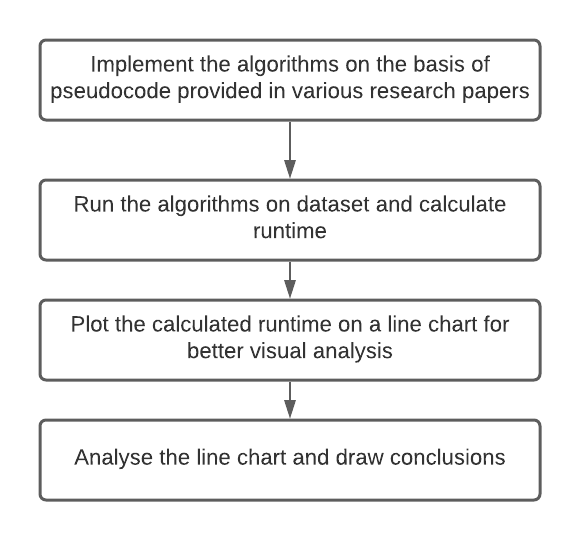
\includegraphics[width=400pt]{work-flow.png}
\captionof{figure}{Performance Analysis of Algorithms: Workflow}

\newpage
\subsection{Theoretical Analysis}
\par
\hspace{1cm}
The runtime of Dijkstra's algorithm in terms of asympotic notation is $O(ElogV)$ where $E$ in the number of edges in graph and $V$ is the number of vertices. In worst case $E$ can be $V*(V-1)/2$. So we can say that runtime is quadratic in terms of number of vertices multiply by log factor.
\\
\par
\hspace{1cm}
The A* algorithm is modification over Dijkstra with addition of heuristic. So if $g$ is a time to calculate value of heuristic in for single vertex then the runtime comes out to be $O((E+g)log(V+g))$ where $E$ in the number of edges in graph and $V$ is the number of vertices. In worst case $E$ can be $V*(V-1)/2$. The runtime is asymptotically same as original graph but A* performs smart search. It eliminates many of the edges during the search which eventually reduces search space to greate margin.
\\
\par
\hspace{1cm}
The HPA* algorithm is just A* running over abstract graph of original graph. Number of vertices in abstract graph are depends on clustering method used. In terms of asymptotic notations the number of vertices in abstract graph may be equal to original graph so it's runtime come out to be same as A* i.e. $O(l*(E+g)log(V+g))$ where $l$ number of levels of hierarchy.
\\
\par
\hspace{1cm}
From the above analysis it can be seen that all three algorithms are having almost same runtime on paper and it is better to test them on real dataset to use for practical applications.

\newpage
 
\subsection{Practical Runtimes}
\begin{enumerate}
\item Maps are rectangular grids which can be represented by $length*width$.
\item All maps are having different structure, that is out of several maps of same type one/two maps are chosen for testing.
\item Runtime is averaged over multiple iterations for different pairs of source and destination.
\item Runtimes are in milli seconds.
\end{enumerate}
\par
\subsubsection{Tabular Form}
\begin{table}[h!]
 \caption{Performance Data}
\begin{center}
\begin{tabular}{| c | c | c | c | c |}
\hline
Sr. No. & Map Size & Dijkstra & A* & HPA* \\
\hline
1 & 49x49 & 1.342 & 0.000 & 0.000 \\
2 & 288x225 & 48.809 & 1.199 & 0.202 \\
3 & 257x320 & 48.998 & 1.499 & 1.496 \\
4 & 256x260 & 22.004 & 25.007 & 3.000 \\
5 & 193x261 & 29.008 & 16.000 & 1.001 \\
6 & 512x518 & 10.010 & 0.000 & 1.955 \\
7 & 193x177 & 26.004 & 0.000 & 0.000 \\
8 & 328x241 & 12.000 & 47.013 & 1.961 \\
9 & 350x310 & 11.999 & 22.999 & 0.000 \\
10 & 77x93 & 1.001 & 0.000 & 0.000 \\
11 & 417x288 & 21.507 & 7.505 & 0.000 \\
12 & 432x288 & 21.045 & 5.008 & 1.000 \\
13 & 876x408 & 84.003 & 122.499 & 0.999 \\
14 & 257x257 & 0.999 & 4.000 & 1.007 \\
15 & 593x401 & 31.004 & 40.002 & 0.000 \\
16 & 649x403 & 18.995 & 1.000 & 0.999 \\
17 & 658x297 & 16.757 & 13.000 & 0.998 \\
18 & 258x258 & 21.004 & 0.997 & 0.997 \\
\hline
\end{tabular}
\end{center}
\end{table}
\vspace{1cm}
\subsubsection{Graphical Analysis}
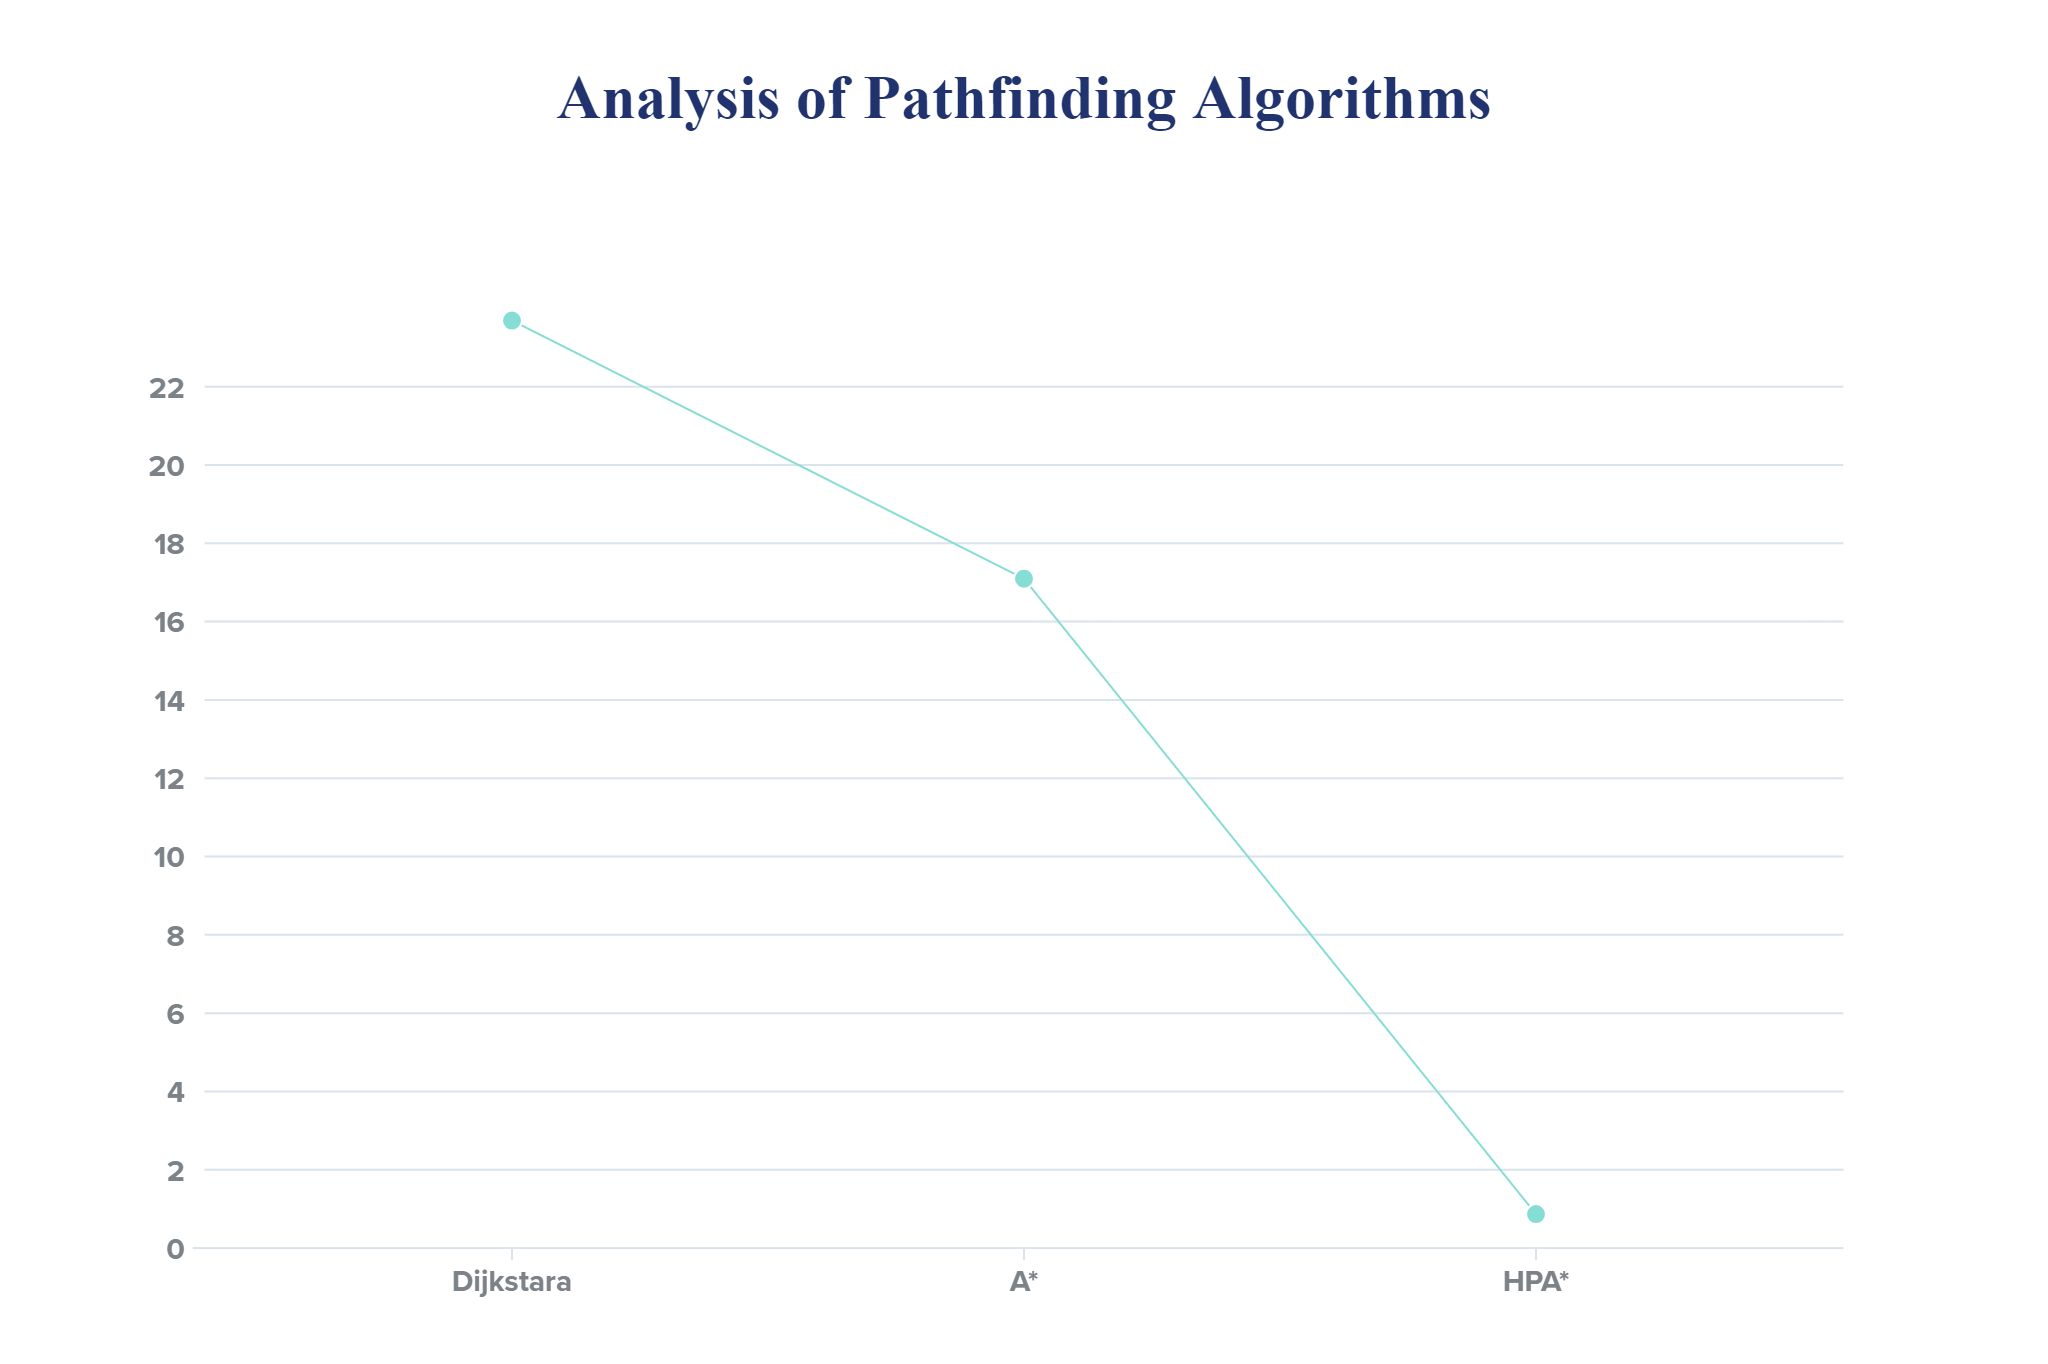
\includegraphics[width=400pt]{analysis-graph.png}
\captionof{figure}{Analysis Graph - It can be observed that Dijkstra's algorithm is constliest algorithm to in pathfinding, while HPA* is the fastest when averaged over dataset.}
\vspace{1cm}
\subsubsection{Result Analysis}
\par From the above results, out of 18 maps tested, it can be seen that A* performed well over Dijkstra in 12 cases while HPA* performed well over A* in 17 cases. It is observed that A* is good replacement over Dijkstra in the cases when heuristic works in favor of path, and HPA* is also good replcement over A* (provided memory requirements of HPA* should be fulfilled) for the application of algorithms in modern computer games.




			
		

% \newpage
% \section{Results}
% \subsection{Data}
% \begin{table}[h!]
% \centering
% \caption{Data Table}
% \begin{tabular}{|l|l|l|}
% \hline
% S.No &Data set  &size  \\ \hline
% 1 &KDD1998  &43.5 MB  \\ \hline
%  2& KDD 1999 &75.3 MB  \\ \hline
% \end{tabular}
% %\caption{Data Table}
% \label{my-label}
% \end{table}
% \subsection{Implementation Results}
% 
\includegraphics[scale=0.5]{pict}
% \captionof{figure}{This is placeholder image: Result of KDD 1998 dataset}
% 
\includegraphics[scale=0.5]{pict}
% \captionof{figure}{This is placeholder image: Result of KDD 1999 dataset}
\newpage
\begin{center}
\section{CONCLUSION and FUTURE WORK}
\end{center}
\par \hspace{1cm}
Despite pathfinding is one of the most common classical problem, the comparison of these algorithms on real world dataset haven't been done yet. In this work I have presented their performance comparison on real-world game dataset and it can be observed that HPA* is best choice in almost all of the cases. A* is good choice in most of the cases but Dijkstra outperforms it when heuristic doesn't work very well.
\\
\par \hspace{1cm} HPA* is not that much explored algorithm compared to Dijkstra's and A*. This algorithm has tendency to replace many traditional algorithms. The path can be made near-optimal using multiple levels of hierarchy and also these algorithm perform very well in case of online search as we need to update graph only for two clusers (source and destination).
\\
 \par \hspace{1cm} As already mentioned, lot of work has been done on Dijkstra and A*. HPA* has lot more potential. This seminar work doesn't calculate the path length which is founded by three algorithms. So another analysis may include path length comparison of three algorithms on the real-game dataset as it is equally important to find optimal path along with efficient runtime. 
\\

\newpage
%
%\bibliography{biblio}
\addcontentsline{toc}{section}{References}
\bibliographystyle{plain}

\begin{thebibliography}{21}

\bibitem{Paper1} E. Dijkstra, A note on two problems in connexion with graphs, Nu777 merische  Mathematik 1 (1959) 269–271

\bibitem{Paper2} Javaid, M.A. Understanding Dijkstra Algorithm. SSRN Electron. J. 2013.

\bibitem{Paper3} Shu-Xi, W. The improved dijkstra’s shortest path algorithm and its application. Procedia Eng. 2012,29, 1186–1190

\bibitem{Paper4} Eneh, A. H., \& Arinze, U. C. (2017). Comparative Analysis and Implementation of Dijkstra's Shortest Path Algorithm For Emergency Response and Logistic Planning. Nigerian Journal of 
Technology, Vol. 36 No. 3 (2017)

\bibitem{Paper5} Foed, D., Ghifari, A., Kusuma, M. B., Hanafiah, N., \& Ganuwan, E. (2021). A Systematic Literature Review of A* Pathfinding. Procedia Computer Science, 179, 507–514

\bibitem{Paper6}  Cui, Xiao and Shi, Hao (2011) A*-based Pathfinding in Modern Computer Games. International Journal of Computer Science and Network Security, 11 (1). pp. 125-130. ISSN 1738-7906

\bibitem{Paper7}  Ade Candra, Mohammad Andri Budiman, \& Rahmat Irfan Pohan. (2020). Application of A Star Algorithm on Pathfinding Game. Journal of Physics: Conference Series, 1898.

\bibitem{Paper8}  Alija, A.S. Analysis of Djikstra’s and A* Algorithm to Find the Shortest Path. Master’s Thesis, Universiti TunHussein Onn Malaysia, Johor, Malaysia, September 2015.

\bibitem{Paper9} Ma, H., Koenig, S., Ayanian, N., Cohen, L., Honig, W., Kumar, T. K. S., Uras, T., and Xu, H. 2016a. Overview: Generalizations of multi-agent path finding to real-world scenarios. In WOMP Workshop at IJCAI.

\bibitem{Paper10} Botea A, Muller M, and Jonathan S. Near optimal hierarchical path-finding. J Game Dev 2004

\end{thebibliography}


\end{document}

